%%%%%%%%%%%%%%%%%%%%%%%%%%%%%%%%%%%%%%%%%
% University/School Laboratory Report
% LaTeX Template
% Version 3.1 (25/3/14)
%
% This template has been downloaded from:
% http://www.LaTeXTemplates.com
%
% Original author:
% Linux and Unix Users Group at Virginia Tech Wiki 
% (https://vtluug.org/wiki/Example_LaTeX_chem_lab_report)
%
% License:
% CC BY-NC-SA 3.0 (http://creativecommons.org/licenses/by-nc-sa/3.0/)
%
%%%%%%%%%%%%%%%%%%%%%%%%%%%%%%%%%%%%%%%%%

%----------------------------------------------------------------------------------------
%	PACKAGES AND DOCUMENT CONFIGURATIONS
%----------------------------------------------------------------------------------------

\documentclass{article}

%\usepackage[version=3]{mhchem} % Package for chemical equation typesetting
%\usepackage{siunitx} % Provides the \SI{}{} and \si{} command for typesetting SI units
\usepackage{graphicx} % Required for the inclusion of images
\usepackage[section]{placeins}
\usepackage{booktabs} % For prettier tables
\usepackage{float} % To control positions of e.g. tables or figures
\usepackage[colorlinks]{hyperref} % To color blocks of text 
\usepackage[dvipsnames]{xcolor} % More color options (see Wikibooks)  
\usepackage{changepage}
%\usepackage[dvipdfmx]{graphicx}
%\usepackage{bmpsize} % Added at some point but now (June-16) it seems to do nothing
%\usepackage{natbib} % Required to change bibliography style to APA
%\usepackage{amsmath} % Required for some math elements 

\graphicspath{{home/totta/Ef\_RNAseq/figures/}}
\setlength\parindent{0pt} % Removes all indentation from paragraphs

\renewcommand{\labelenumi}{\alph{enumi}.} % Make numbering in the enumerate environment by letter rather than number (e.g. section 6)

%\usepackage{times} % Uncomment to use the Times New Roman font
%----------------------------------------------------------------------------------------
%	DOCUMENT INFORMATION
%----------------------------------------------------------------------------------------

\title{Overview of dual RNA-seq data from \textit{Eimeria falciformis} infected \textit{Mus musculus}} % Title

\author{Totta \textsc{Kasemo}} % Author name

\date{\today} % Date for the report

\begin{document}

\maketitle % Insert the title, author and date

\begin{center}
\begin{tabular}{l r}
%Date Performed: & January 1, 2012 \\ % Date the experiment was performed
%Partners: & James Smith \\ % Partner names
%& Mary Smith \\
%Instructor: & Professor Smith % Instructor/supervisor
\end{tabular}
\end{center}

% If you wish to include an abstract, uncomment the lines below
% \begin{abstract}
% Abstract text
% \end{abstract}

%----------------------------------------------------------------------------------------
%	SECTION 1
%----------------------------------------------------------------------------------------

\section{Objective}

This summary table of reads generated in each sample.....

%\begin{center}\ce{}\end{center}

%----------------------------------------------------------------------------------------
%	SECTION 2 
%----------------------------------------------------------------------------------------

\section{Table of reads per sample}
% latex table generated in R 3.2.2 by xtable 1.8-2 package
% Wed Mar  2 14:36:30 2016
\setlength{\tabcolsep}{10pt}
\begin{table}[H]
\centering 
\caption{Transcripts per sample listed for \textit{E. falciformis} and mouse. Percentage of
	\textit{E. falciformis} transcripts and number of \textit{E. falciformis} genes are alo shown. 
	Gray indicates that samples are excluded from analysis (see Methods for details).}
\begin{tabular}{*5l}    \toprule
Samples  & Mouse 	& \textit{E. falciformis}  & Percent			& \#\textit{E.falciformis} \\
	& trancripts	& transcripts   	 & \textit{E. falciformis}	& genes \\ \midrule
NMRI\_oocysts\_rep1 & 11676.000 & 108477484.000 & 99.989 & 5734.000 \\ 
NMRI\_oocysts\_rep2 & 19024.000 & 126543533.000 & 99.985 & 5774.000 \\ 
NMRI\_sporozoites\_rep1 & 13800.000 & 92259539.000 & 99.985 & 5808.000 \\ 
NMRI\_sporozoites\_rep2 & 8702.000 & 21508353.000 & 99.960 & 5564.000 \\ 
NMRI\_1stInf\_7dpi\_rep1 & 12532238.000 & 79648900.000 & 86.405 & 5894.000 \\ 
NMRI\_1stInf\_7dpi\_rep2 & 94310278.000 & 154343046.000 & 62.072 & 5897.000 \\ 
NMRI\_1stInf\_5dpi\_rep3 & 334671421.000 & 54022504.000 & 13.899 & 5794.000 \\ 
NMRI\_2ndInf\_7dpi\_rep1 & 97221189.000 & 9927803.000 & 9.265 & 5865.000 \\ 
NMRI\_1stInf\_5dpi\_rep1 & 204647381.000 & 18549727.000 & 8.311 & 5739.000 \\ 
C57BL6\_1stInf\_5dpi\_rep2 & 32887009.000 & 250954.000 & 0.757 & 3946.000 \\ 
	{\color{Gray}NMRI\_2ndInf\_5dpi\_rep1} & {\color{Gray} 589643389.000} & {\color{Gray}3752923.000} & {\color{Gray} 0.632} &  {\color{Gray}5602.000} \\ 
NMRI\_1stInf\_5dpi\_rep2 & 316721928.000 & 1609009.000 & 0.505 & 5439.000 \\ 
C57BL6\_2ndInf\_5dpi\_rep1 & 62053975.000 & 311900.000 & 0.500 & 4610.000 \\ 
	{\color{Gray}NMRI\_1stInf\_3dpi\_rep1} & {\color{Gray}209723287.000} &  {\color{Gray}815820.000} &  {\color{Gray}0.388} &  {\color{Gray}5466.000} \\ 
C57BL6\_1stInf\_5dpi\_rep1 & 65523435.000 & 217606.000 & 0.331 & 4259.000 \\ 
Rag\_2ndInf\_5dpi\_rep1 & 85288323.000 & 224273.000 & 0.262 & 4251.000 \\ 
Rag\_1stInf\_5dpi\_rep2 & 57192380.000 & 113673.000 & 0.198 & 2969.000 \\ 
NMRI\_1stInf\_3dpi\_rep2 & 515516785.000 & 903330.000 & 0.175 & 5101.000 \\ 
Rag\_1stInf\_5dpi\_rep1 & 71173382.000 & 73445.000 & 0.103 & 2748.000 \\ 
NMRI\_2ndInf\_7dpi\_rep2 & 122999109.000 & 46700.000 & 0.038 & 2174.000 \\ 
NMRI\_2ndInf\_3dpi\_rep2 & 106446839.000 & 34699.000 & 0.033 & 1901.000 \\ 
	 {\color{Gray}NMRI\_1stInf\_0dpi\_rep1} &  {\color{Gray}229165002.000} & {\color{Gray} 31459.000} &  {\color{Gray}0.014} & {\color{Gray} 1380.000} \\ 
NMRI\_2ndInf\_5dpi\_rep2 & 113957667.000 & 12692.000 & 0.011 & 539.000 \\ 
NMRI\_2ndInf\_3dpi\_rep1 & 91352242.000 & 5355.000 & 0.006 & 121.000 \\ 
NMRI\_2ndInf\_0dpi\_rep2 & 90681785.000 & 3738.000 & 0.004 & 62.000 \\ 
Rag\_0dpi\_rep1 & 43414004.000 & 474.000 & 0.001 & 2.000 \\ 
C57BL6\_0dpi\_rep1 & 53877840.000 & 491.000 & 0.001 & 2.000 \\ 
C57BL6\_0dpi\_rep2 & 76753491.000 & 657.000 & 0.001 & 2.000 \\ 
Rag\_0dpi\_rep2 & 80702547.000 & 730.000 & 0.001 & 3.000 \\ 
NMRI\_2ndInf\_0dpi\_rep1 & 285032128.000 & 326.000 & 0.000 & 2.000 \\ 
\bottomrule
\hline
\end{tabular}
\end{table}




%%%%%%%%%%%%%%%%%%%%%%%%%%%%%%%%%%%%%%%%%%%%%%%%%%%%%%%%%%%%%%%%%%%%%%%%%%
%% 	OVERVIEW READS PER SAMPLE, LAYOT AS EXPERIMENTAL OVERVIEW
%%%%%%%%%%%%%%%%%%%%%%%%%%%%%%%%%%%%%%%%%%%%%%%%%%%%%%%%%%%%%%%%%%%%%%%%%%
\section{Experimental overview with transcripts per sample}
	\setlength{\tabcolsep}{14pt}
	\begin{table}[H]
	\begin{center}
	\caption{Replicate average transcripts numbers as order of magnitude for \textit{E. falciformis}
		(first) and mouse (second) and experimental overview. Columns represent different mouse strains
		used (NMRI, C57BL/6 and Rag1-/-). Rows are different timepoints post infection or parasite life cycle 
		stages. The upper part shows data for first infection, and oocyst and sporozoite data. The lower part 
		shows data for challange infection. Averages were calculated after sample exclusions (see Methods). 
		For exact values, see Table 1.}
\begin{tabular}{*4l}    \toprule
\textit{Day, 1st infection}  	& NMRI  & C57BL/6  & Rag1-/- \\ \midrule
	0 (control)    & $10^4$ / $10^8$  & $10^2$ / $10^8$  & $10^2$ / $10^7$  \\ %rep1/rep2, NA=no replicate
3  		& $10^5$ / $10^8$ & NA  & NA \\ 
5  		& $10^7$ / $10^8$ & $10^5$ / $10^7$  & $10^5$ / $10^7$ \\
7  		& $10^8$ / $10^7$ & NA  & NA \\ 
Oocysts 	& $10^8$ / NA & NA  & NA \\ 
Sporozoites 	& $10^7$ / NA & NA  & NA \\ \midrule

\textit{Day, 2nd infection}  	\\ \midrule
0 (control)     & $10^3$ / $10^8$  &  NA  & NA  \\ %rep1/rep2, NA=no replicate
3  		& $10^4$ / $10^8$ & NA  & NA \\ 
5  		& $10^4$ / $10^8$ & $10^5$ / $10^7$  & $10^5$ / $10^7$ \\
7  		& $10^6$ / $10^8$ & NA  & NA \\ 
	
	
	\bottomrule
 \hline
\end{tabular}
\end{center}
\end{table}


%%%%%%%%%%%%%%%%%%%%%%%%%%%%%%%%%%%%%%%%%%%%%%%%%%%%%%%%%%%%%%%%%%%%%%%%%%
%% 	MICROARRAY COMPARISON
%%%%%%%%%%%%%%%%%%%%%%%%%%%%%%%%%%%%%%%%%%%%%%%%%%%%%%%%%%%%%%%%%%%%%%%%%%
\section{Transcript distribution and excluding samples}
\subsection{Mouse transcript distributions}
\begin{figure}[H]
\centering
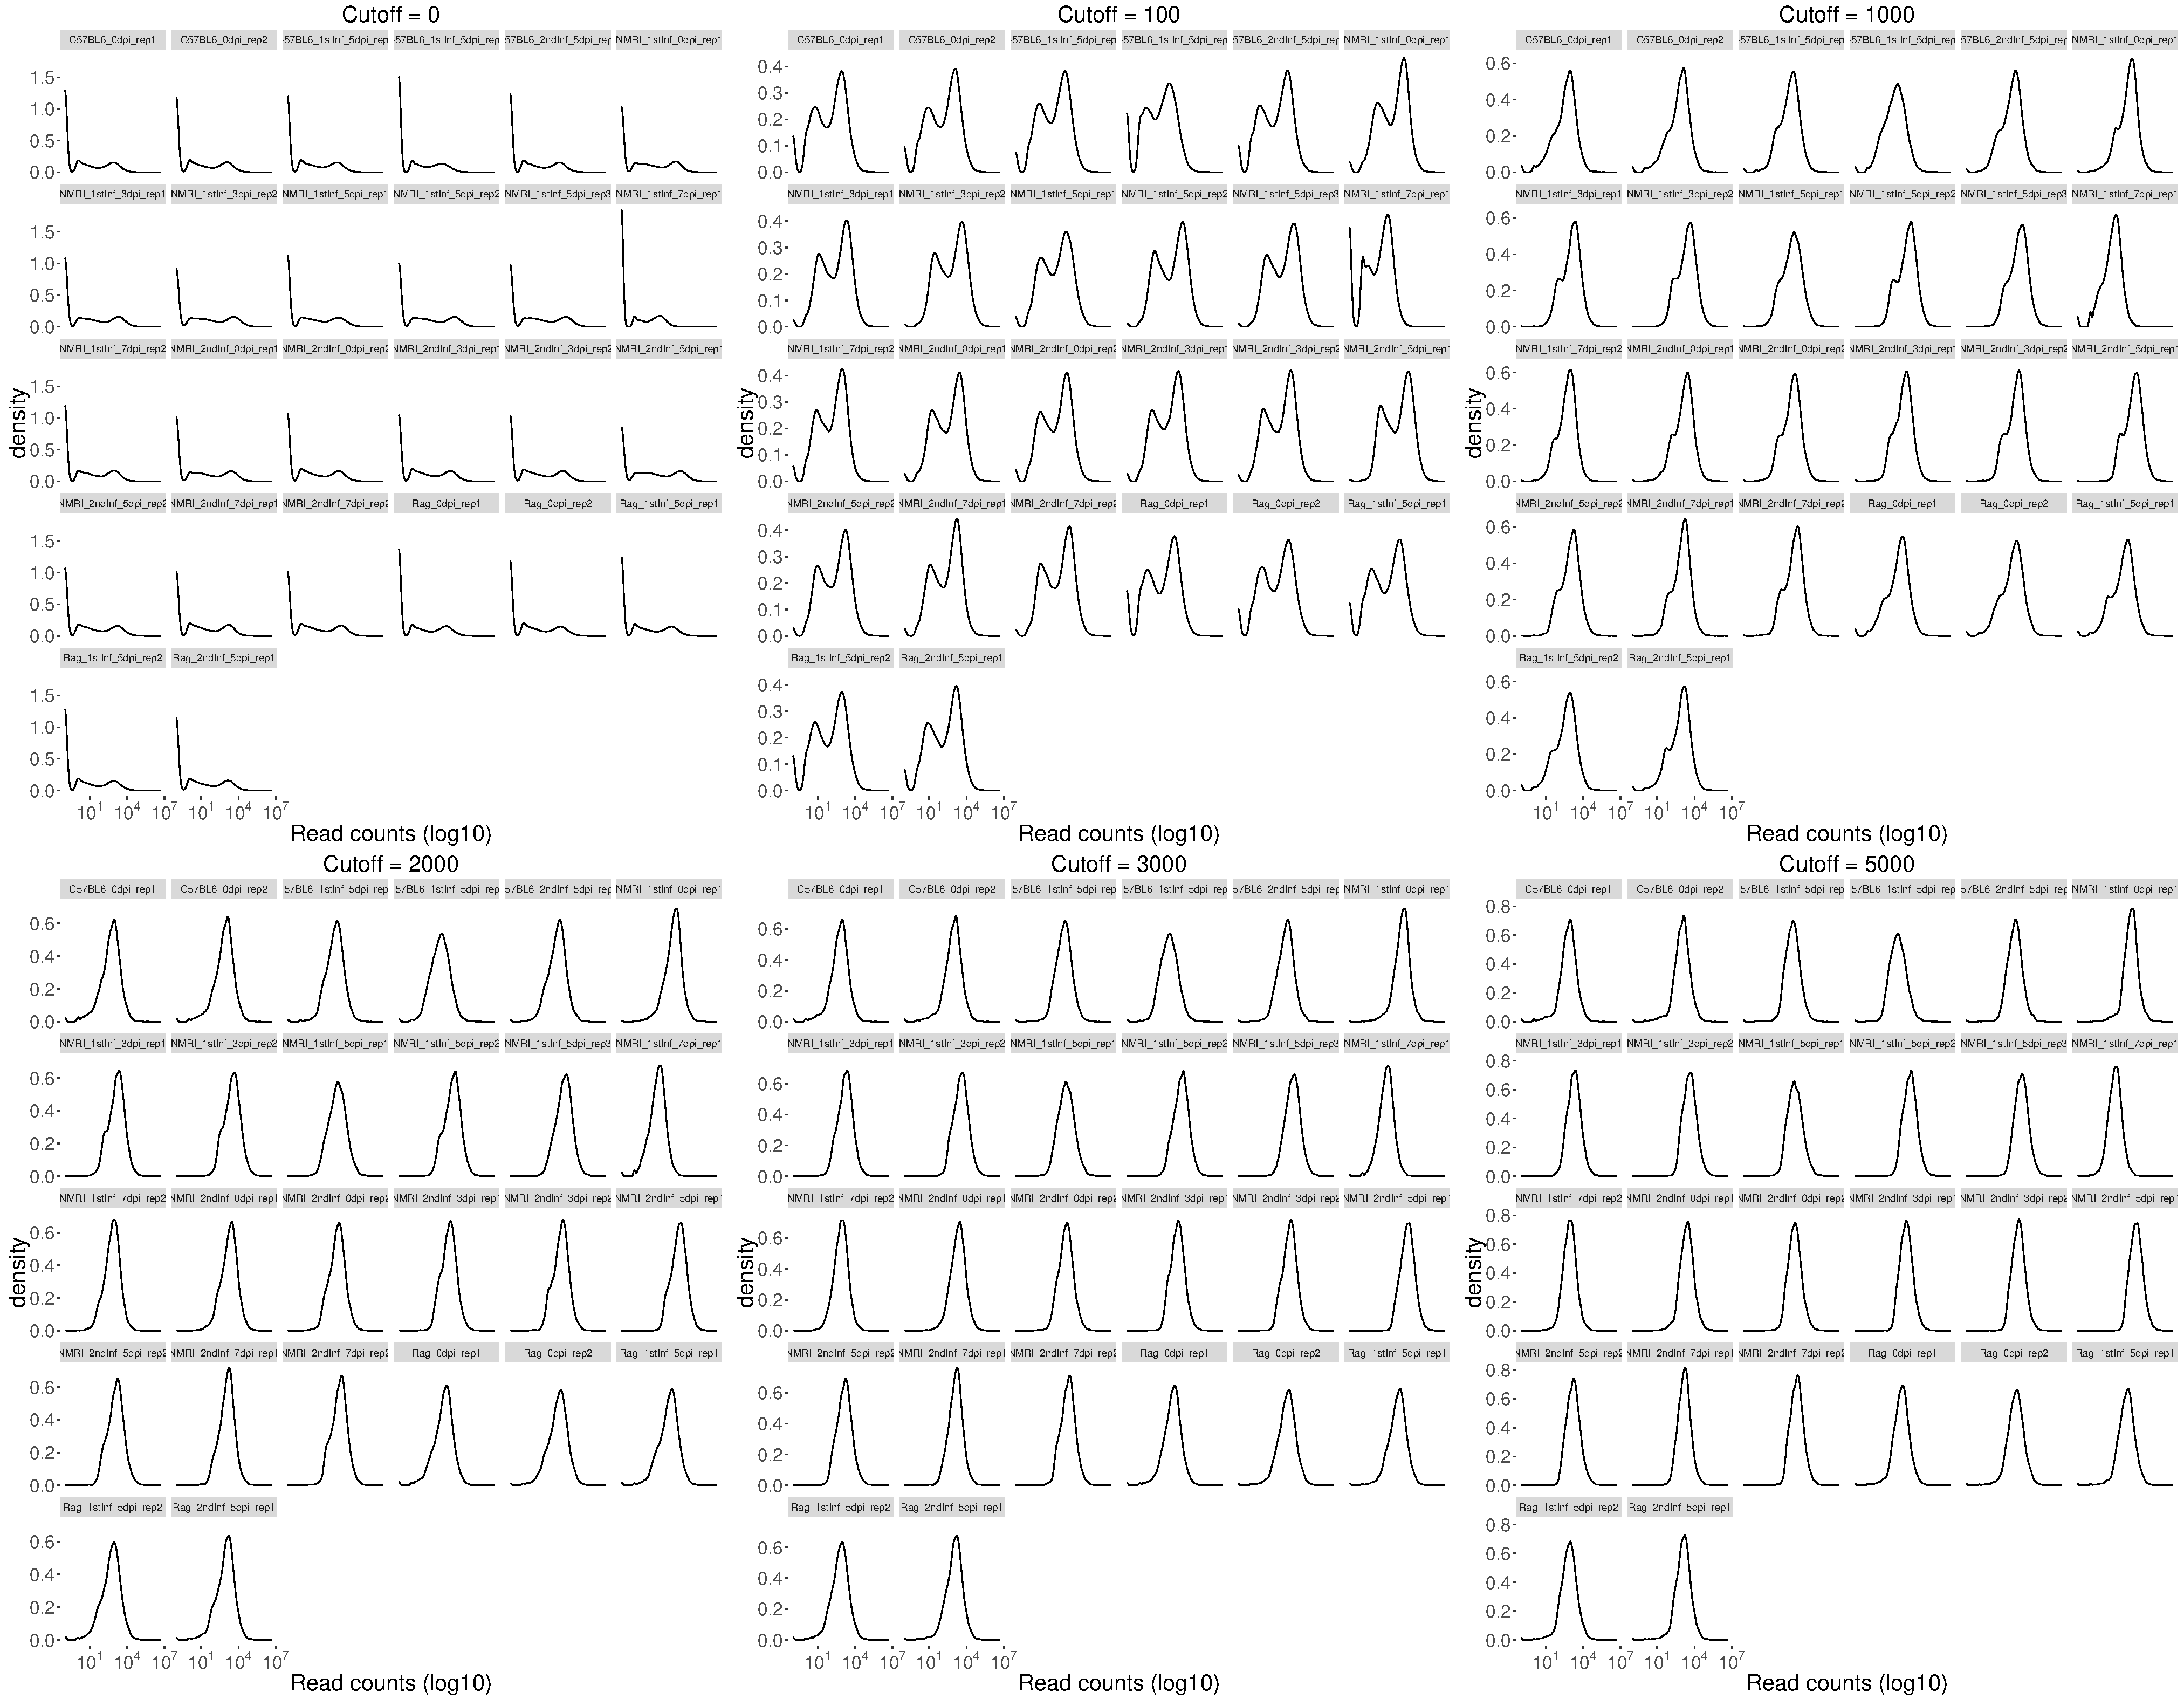
\includegraphics[width=\textwidth]{distributionsMm.pdf}
\caption{Density of transcripts (y-axis) with a specific number of reads mapping (x-axis). 
Density of raw transcripts (not normalised) for all mouse samples. Without any requirement 
(cutoff) for a minimum read coverage per transcript, all samples display a bimodal distribution 
trend and an additional peak at zero by visual inspection. A minimal number of total reads 
(sum for all samples) mapping to one transcript was set (cutoff). For further analysis, a cutoff of
2000 was applied with which for the edgeR anaylsis assumed negative binomial distribution is not 
contradicted. For the density distribution analysis, 0.1 was added to all read values to allow plotting 
density of absent transcripts on a log-scale.}
%\end{center}
\end{figure}

\clearpage
\subsection{\textit{E. falciformis} transcript distributions}
\begin{figure}[H]
\begin{center}
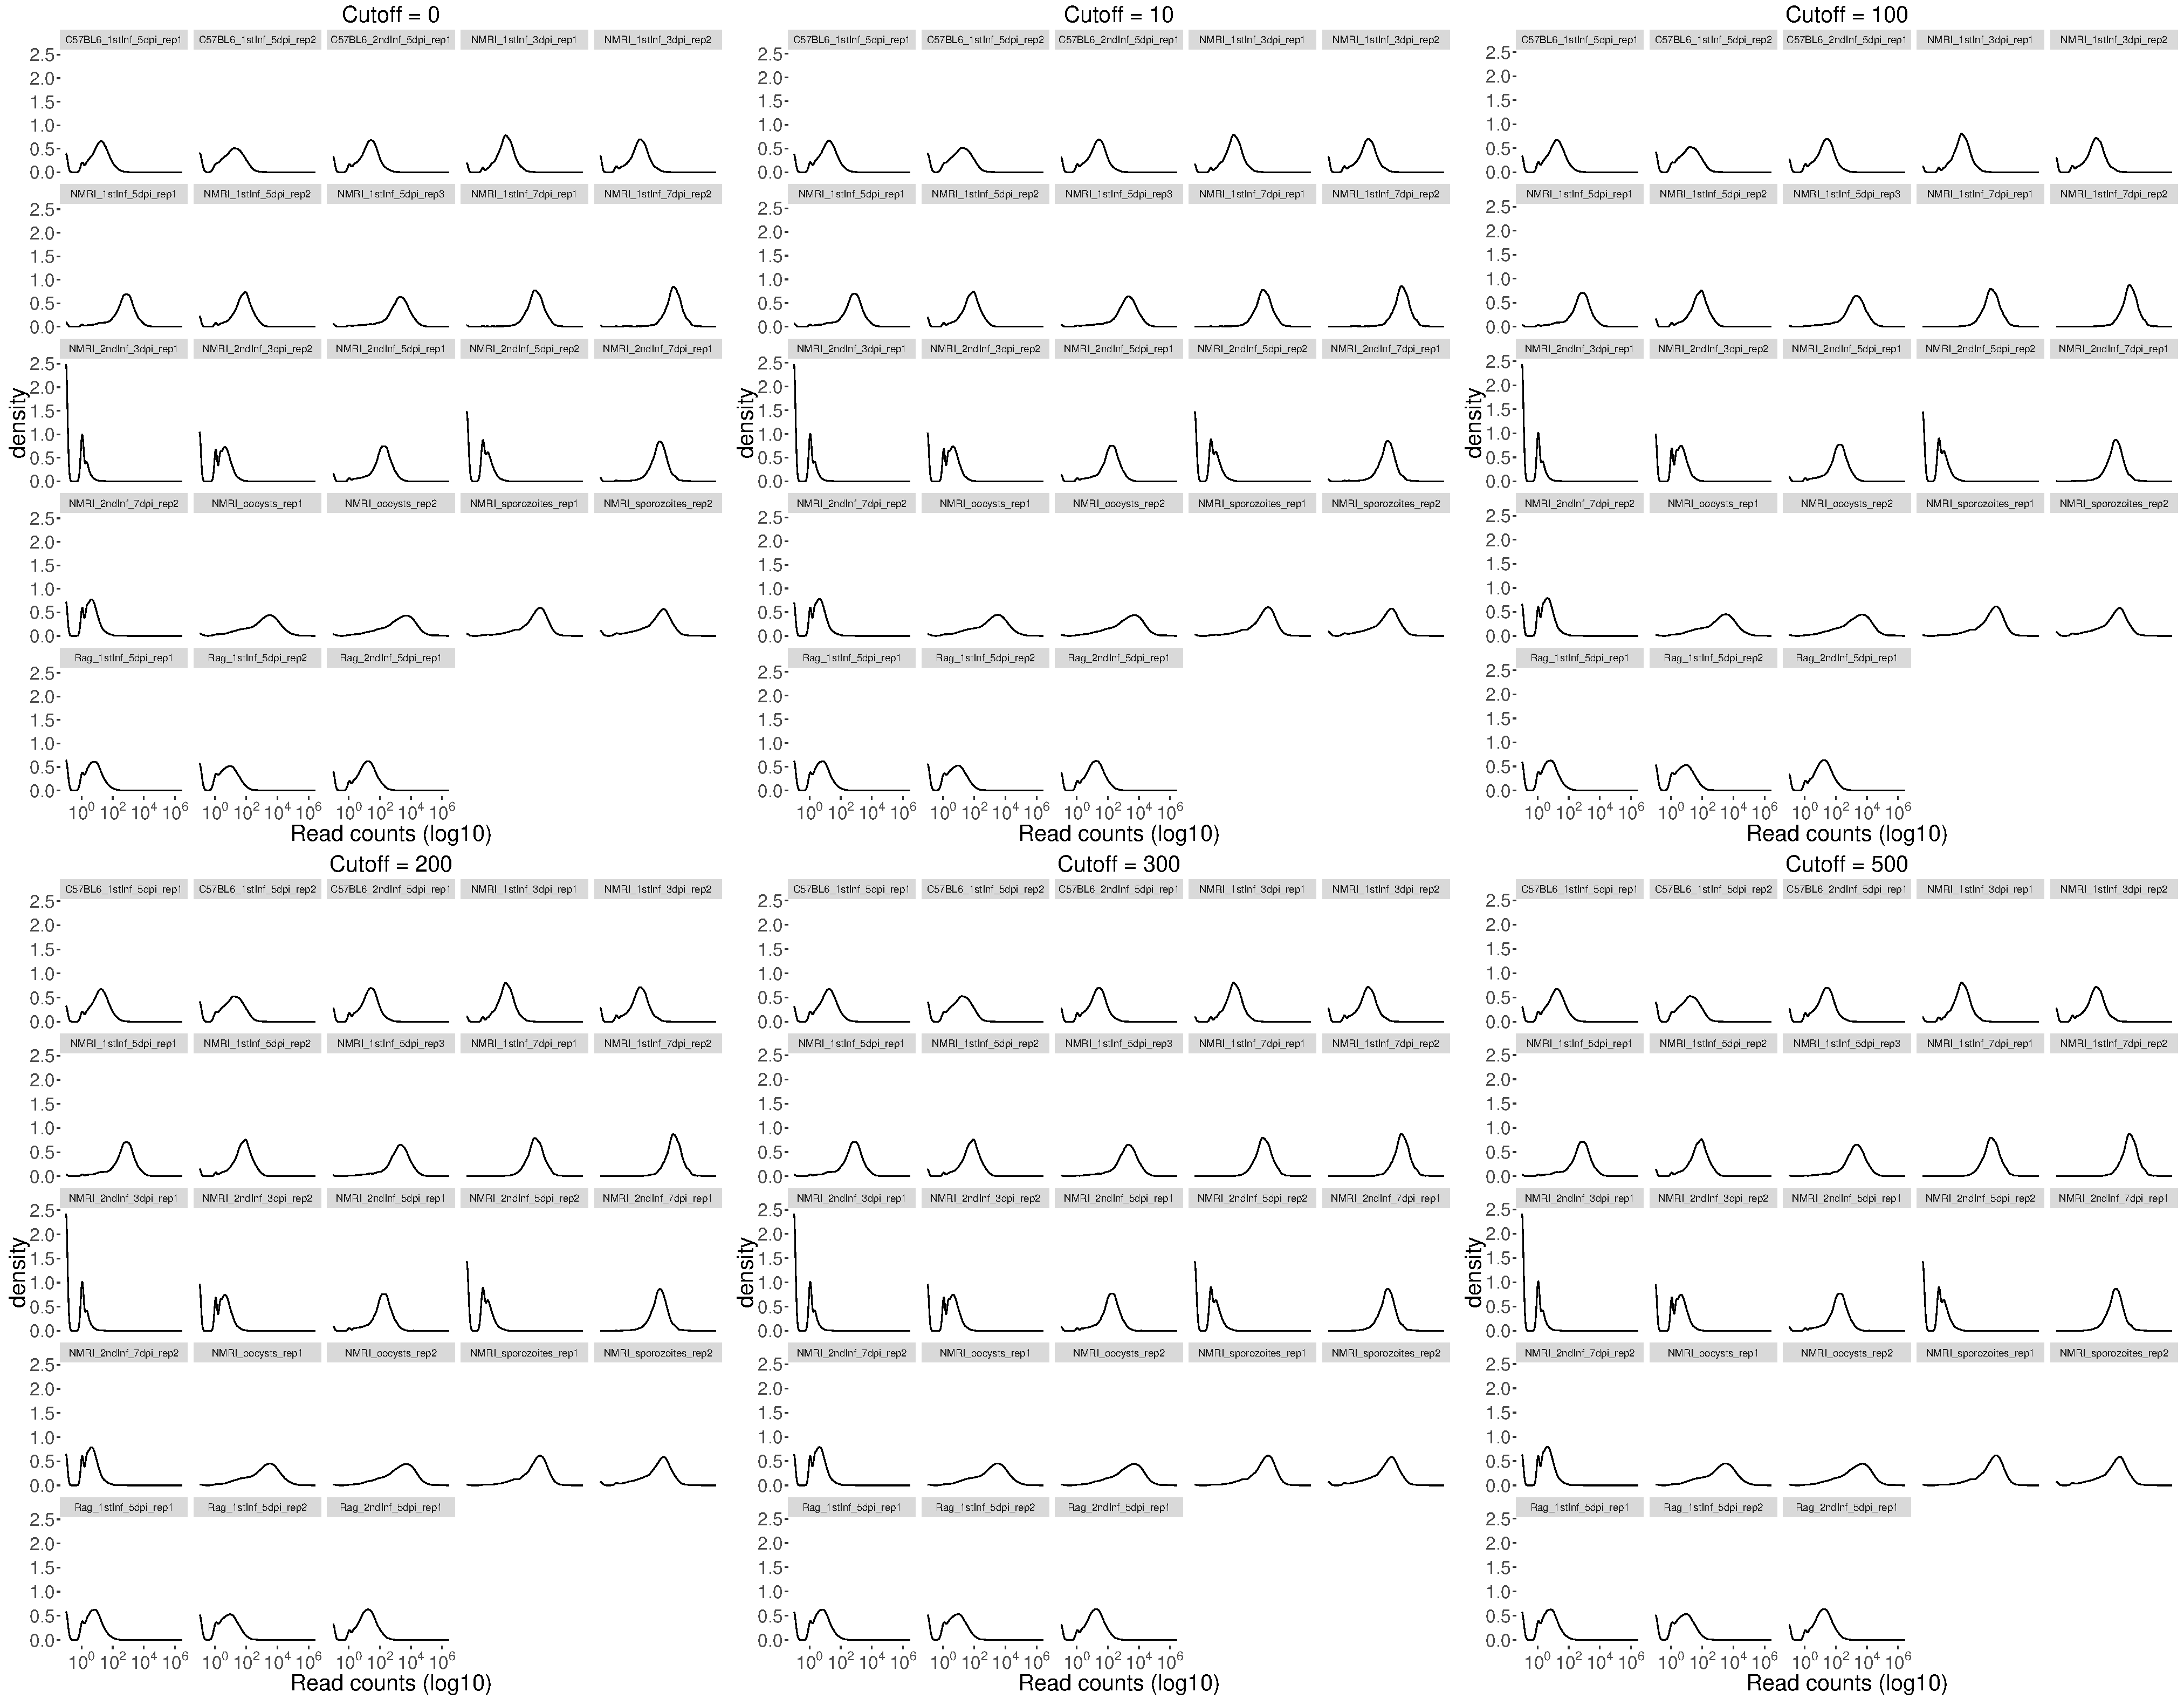
\includegraphics[width=\textwidth]{distributionsEf.pdf}
\caption{Density of transcripts (y-axis) with a specific number of reads mapping (x-axis). 
Density of raw transcripts (not normalised) for all \textit{E. falciformis} samples. Without any
requirement (cutoff) for a minimum read coverage per transcript, most samples do not contradict
the assumed negative binomial distribution. However, two samples clearly do and a cutoff was applied 
to evaluate whether peaks can be removed by excluding transcripts with very low coverage.
The cutoff does not have a large effect on distributions of \textit{E. falciformis} data and therefore 
two samples were removed from further analysis: NMRI\_1st\_3dpi\_rep1 and NMRI\_2nd\_5dpi\_rep1.
	To all read values, 0.1 was added to allow plotting density of absent transcripts on a log-scale.}
\end{center}
\end{figure}

%%%%%%%%%%%%%%%%%%%%%%%%%%%%%%%%%%%%%%%%%%%%%%%%%%%%%%%%%%%%%%%%%%%%%%%%%%
%% 	MICROARRAY COMPARISON
%%%%%%%%%%%%%%%%%%%%%%%%%%%%%%%%%%%%%%%%%%%%%%%%%%%%%%%%%%%%%%%%%%%%%%%%%%
\section{Mouse RNA-seq data compared with mouse microarray data}
%%% figure 1
\begin{figure}[H]
\begin{center}
%\includegraphics[width=\textwidth]{Array144_vs_RNAseqN7.pdf} % Merge 2 plots: RUV and non-RUV 
\caption{Comparison of mouse data from RNA-seq, day 7, (y-axis) and microarray data, day 6 (x-axis, (schmid14)). 
	a. Data normalised with upperquartile method implemented in R package edgeR (version ...). $R^2$ = yy. 
	b. Normalised data as i a. and adjusted with RUV method as implemented in R package RUVseq (version....). 
	$R^2$ = xx. Each axis shows log fold changes compared to control.}
\end{center}
\end{figure}

%%%%%%%%%%%%%%%%%%%%%%%%%%%%%%%%%%%%%%%%%%%%%%%%%%%%%%%%%%%%%%%%%%%%%%%%%%
%% 	MDS ANALYSIS
%%%%%%%%%%%%%%%%%%%%%%%%%%%%%%%%%%%%%%%%%%%%%%%%%%%%%%%%%%%%%%%%%%%%%%%%%%
\section{Analysing variance in data by multidimensional scaling}
\begin{figure}[H]
\begin{center}
	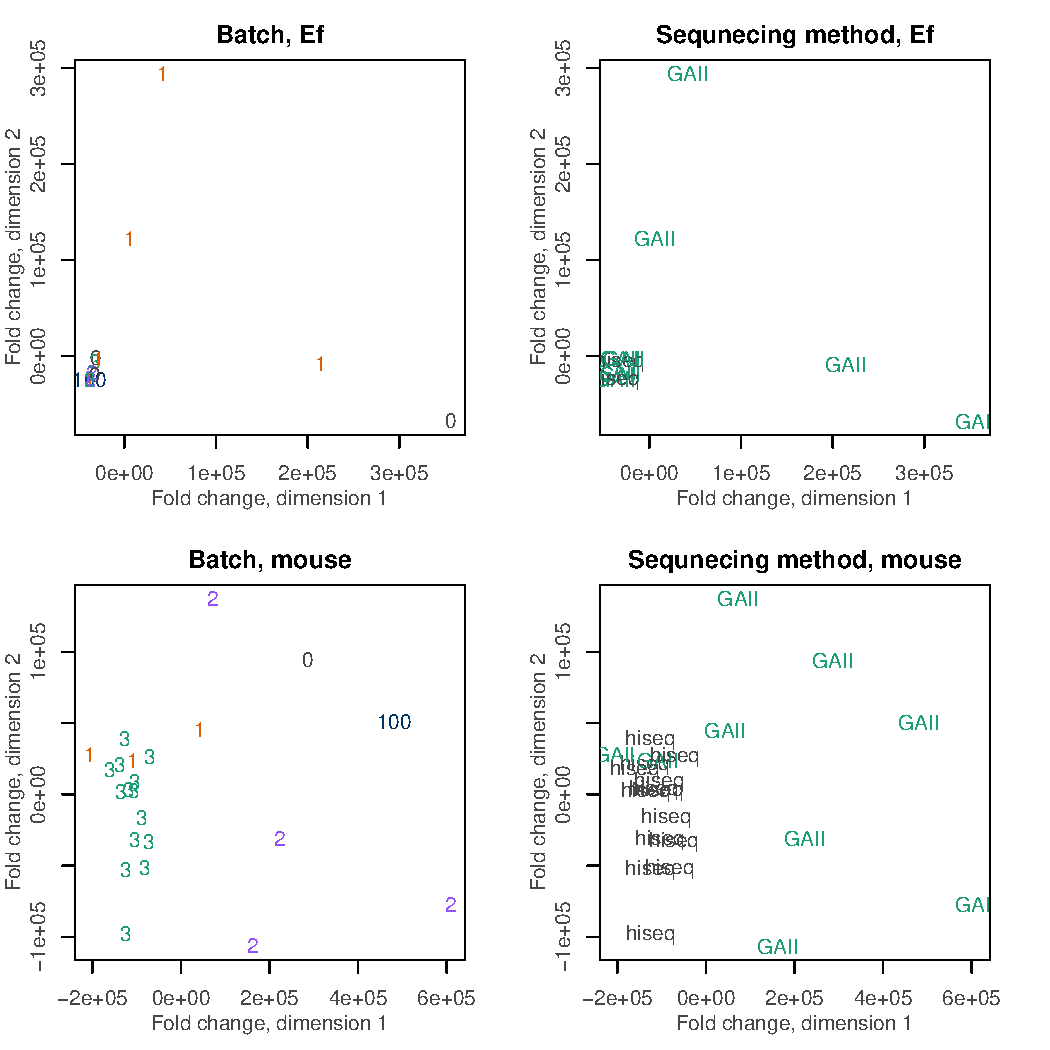
\includegraphics[width=\textwidth]{EfMm_4-mds.pdf} % Include 
	\caption{Multidimensional scaling shows no clear sample pattern due to technical variation. Effect on scaling is visualized 
	for batch (left) and sequencing method (right). Upper panel displays \textit{E. falciformis} data and lower panel mouse data. 
	Distances on plot approximate log2 fold changes. Scaling was done with Euklidean distance and "pairwise" gene selection 
	method as implemented in R package limma (version ...).}
\end{center}
\end{figure}

%%%%%%%%%%%%%%%%%%%%%%%%%%%%%%%%%%%%%%%%%%%%%%%%%%%%%%%%%%%%%%%%%%%%%%%%%%
%% 	NUMBER OF GENES DIFFERENT IN DIFFERENT COMPARISONS	
%%%%%%%%%%%%%%%%%%%%%%%%%%%%%%%%%%%%%%%%%%%%%%%%%%%%%%%%%%%%%%%%%%%%%%%%%%
\clearpage
\section{mRNA abundance differences between different experimental groups}
\setlength{\tabcolsep}{14pt}
\begin{table}[H]
\begin{center}
\caption{\textit{E. falciformis} data overview of pairwise comparisons and number of genes with differently abundant mRNAs 
	per comparison. NMRI followed by number indicates day post infection (e.g. NMRI3 = \textit{E. falciformis} genes from
	NMRI mouse day 3 post infection). Genes with Benjamini-Hochberg corrected p-values \leq0.01 as implemented in edgeR are indluced. 
	ADD MOUSE DATA COLUMN.}
%\label{tab:table3}
\begin{tabular}{*2l}    \toprule
\textit{Comparisons with difference} & Genes different (FDR\leq0.01) \\ \midrule
	NMRI3 vs NMRI5     	& 111  \\
	NMRI3 vs NMRI7  	& 1385 \\ 
	NMRI5 vs NMRI7  	& 1895 \\
	Oocysts vs NMRI3  	& 3310 \\  
	Oocysts vs NMRI5	& 3605 \\ 
	Oocysts vs NMRI7	& 3085 \\ 
	Oocysts vs sporozoites & 3421 \\
	Sporozoites vs NMRI3 	& 1663 \\
	Sporozoites vs NMRI5 	& 1605 \\
	Sporozoites vs NMRI7 	& 2473 \\ 
	NMRI vs C57BL/6 	& 22 \\	\midrule	
\textit{Comparisons, no difference}  	\\ \midrule
	NMRI vs Rag1-/-     & 0 \\
	C57BL/6 vs Rag1-/-  & 0 \\
	NMRI3 1st vs NMRI3 2nd  	    & 0 \\
	NMRI5 1st vs NMRI5 2nd  	    & 0 \\
	NMRI7 1st vs NMRI7 2nd  	    & 0 \\
	C57BL/6 1st vs C57BL/6 2nd (day 5) & 0 \\
	Rag1-/- 1st vs Rag1-/- 2nd (day 5) & 0 \\ \bottomrule
\hline
\end{tabular}
\end{center}
\end{table}
%%%%%%%%%%%%%%%%%%%%%%%%%%%%%%%%%%%%%%%%%%%%%%%%%%%%%%%%%%%%%%%%%%%%%%%%%%
%% 	INPUT TO HEATMAP	
%%%%%%%%%%%%%%%%%%%%%%%%%%%%%%%%%%%%%%%%%%%%%%%%%%%%%%%%%%%%%%%%%%%%%%%%%%
\subsection{Differentially abundant mRNAs used for hierarchical clustering}
\setlength{\tabcolsep}{10pt}
\begin{table}[H]
\begin{adjustwidth}{-10}{}
\begin{center}
	\caption{A selection of differently abundant mRNAs are used for hierarchical clustering of \textit{E. falciformis}
	life cycle relevant genes. In each comparison (see Table 3), the 500 differentially abundant mRNAs with lowest FDR
	are selected. In the next step, the 500 mRNAs from each comparison (or less) are joined (4935 genes) and only 
	unique genes are selected (1618 genes). The 22 genes in the NMRI vs C57BL/6 
	comparison are not included in the \textit{E. falciformis} life cycle analysis.}
\begin{tabular}{*2l}    \toprule
	\textit{Data description} & Number of genes \\ \midrule
	Sum of 1st infection NMRI sample differences	& 4935  \\ 
	(including oocysts and sporozoites)	\\	
	Used in hierarchical clustering (heatmap)  	& 1618 \\ 	\bottomrule	
\hline
\end{tabular}
\end{center}
\end{adjustwidth}
\end{table}
%%%%%%%%%%%%%%%%%%%%%%%%%%%%%%%%%%%%%%%%%%%%%%%%%%%%%%%%%%%%%%%%%%%%%%%%%%
%% 	HEATMAPS
%%%%%%%%%%%%%%%%%%%%%%%%%%%%%%%%%%%%%%%%%%%%%%%%%%%%%%%%%%%%%%%%%%%%%%%%%%
\section{Hierarchical clustering of genes different depending on time post infection}
\begin{figure}[H]
\begin{center}
\includegraphics[width=\textwidth]{Ef_most_sig_lifecycle_heatmapi.pdf}  
	\caption{\textit{E. falciformis} with Euklidean distance .........as implemented in R package limma.}
\end{center}
\end{figure}


\end{document}

